\documentclass{beamer}
\usepackage[latin1, utf8]{inputenc}
\usepackage[francais]{babel}
\usepackage{wrapfig}
\usepackage{framed}
%****
\usepackage{multimedia}
%\usepackage{media9}
\usepackage{hyperref}

\useoutertheme[height=0pt,left]{sidebar}
\usecolortheme{seahorse}
\setbeamercolor*{titlelike}{parent=structure}
\useinnertheme{circles}
\setbeamertemplate{frametitle}[default][right]

%\title{Les robots ressemblant à l'humain sont-ils vraiment utiles ?}
\title{\textsc{L'imitation de l'être humain doit-elle être un objectif ?}}
\author{Christian LASSERRE \& Théophile GUILBAUD}
%\institute{ENSEIRB-MATMECA}
\date{}

\begin{document}
\begin{frame}
  \titlepage
      {
        \vspace*{-1cm}
        \begin{center} 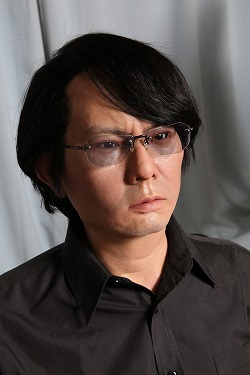
\includegraphics[width=35mm]{data/HI-4} \end{center}
      }
\end{frame}

\begin{frame}
  \tableofcontents
\end{frame}

\section{Ressemblance}
\begin{frame}{RESSEMBLANCE}
  ``Quel rôle joue l’imitation la culture et quelle est son importance pour le savoir anthropologique ? Ce texte souligne quelques voies d’approche possibles. L’imitation peut être envisagée comme une stratégie parodique, une compétence cognitive, un moyen de \colorbox{yellow}{transmission culturelle}, un principe de l’\colorbox{yellow}{apprentissage social} ou un \colorbox{yellow}{mécanisme d’adaptation}. Les processus d’imitation impliquent des \colorbox{pink}{compétences cognitives spécifiques} et s’inscrivent dans des \colorbox{pink}{contextes sociaux et culturels déterminés}. Parce qu’ils se situent à la charnière des sphères du biologique et du culturel, ces processus font partie du projet anthropologique qui cherche à comprendre à la fois l’unité cognitive de l’homme et la diversité de ses réalisations culturelles.''
  ~\\~\\
  {\small Nélia Dias, dans ``Imitation et Anthropologie''}  
\end{frame}

\subsection{Le(s) Géminoide(s)}
\begin{frame}{Hiroshi Ishiguro}
  Roboticien japonais, directeur du Intelligent Robotics Laboratory, 
  qui dépend du ``Department of Adaptive Machine'' à l'Université d'Osaka, 
  au Japon.\\~\\
  Exemple de publications :
  \begin{itemize}
  \item Acquiring 3-D structure by controlling visual attention of a mobile 
    robot (Robotics \& Automation, 05/1990)
  \item Cognitive developmental robotics as a new paradigm for the design 
    of humanoid robots (Robotics and Autonomous System, 04/2001)
  \item Natural Behavior Generation for Humanoid Robot (Robotics and Autonomous System, 12/2004)
  \item  A humanoid robot that pretends to listen to route guidance from a 
    human (Autonomous Robots, 01/2007)
    %% \item Group attention control for communication robot, Masahiro Shiomi, 
    %%   Takayuki Kanda, Satoshi Koizumi, Hiroshi Ishiguro, Norihiro Hagita, 
    %%   International Journal of Humanoid Robotics, Vol.5, Issue 4, pp.587-608, 
    %%   2008.12, Papers
    %% \item ``Could I Have a Word?'': Effects of Robot’s Whisper, Masahiro shiomi, 
    %%   Kayako Nakagawa, Reo Matsumura, Kazuhiko Shinozawa, Hiroshi Ishiguro,
    %%   Norihiro Hagita, Proceedings of International Conference on RObots and 
    %%   Systems (IROS2010), pp.3899-3904, 2010.10, Conference Report / Oral Presentation
    %% \item Motion Design of Interactive Small Humanoid Robot with Visual Illusion, 
    %%   Kurima Sakai, Hidenobu Sumioka, Takashi Minato, Shuichi Nishio, 
    %%   Hiroshi Ishiguro, International Journal of Innovative Computing, 
    %%   Information and Control, vol. 9, no. 12 'pp. 1–10, 2013.12, Papers
  \end{itemize}
\end{frame}

\begin{frame}
  Crée le HIL (``Hiroshi Ishiguro Laboratory'') ayant pour mission:\\~\\
  ``{
    \footnotesize  
    The end of the information age will coincide with the beginning of the 
    robot age. However, we will not soon see a world in which humans and 
    androids walk the streets together, like in movies or cartoons; instead, 
    information technology and robotics will \colorbox{yellow}{gradually 
      fuse so that people will likely only notice when robot technology is already in use in 
      various locations}.\\
    ~\\

    Our role will be \colorbox{yellow}{to lead this integration of information and robotics 
      technologies by constantly proposing new scientific and technological 
      concepts.}
    Toward this, knowledge of \colorbox{yellow}{art and philosophy will be invaluable}.
    Technology has made art ``reproducible''; likewise, artistic sense has 
    contributed to the formation of new technologies, and artistic endeavors
    themselves are supported by philosophical contemplation and analysis.\\
    ~\\
    
    Hereafter, human societies will continue to change due to ``informationization'' 
    and robotization; in this ever-changing setting, artistic activities and philosophical 
    speculation will allow us to comprehend the \colorbox{yellow}{essential natures of humans and society}, 
    so that we can produce truly novel science and technological innovations in a 
    research space which lies beyond current notions of ``fields'' and boundaries of existing knowledge.
  }''

\end{frame}

\subsection{Caractéristiques}
\begin{frame}{Geminoide HI-4}
  \begin{figure}
    \centering
    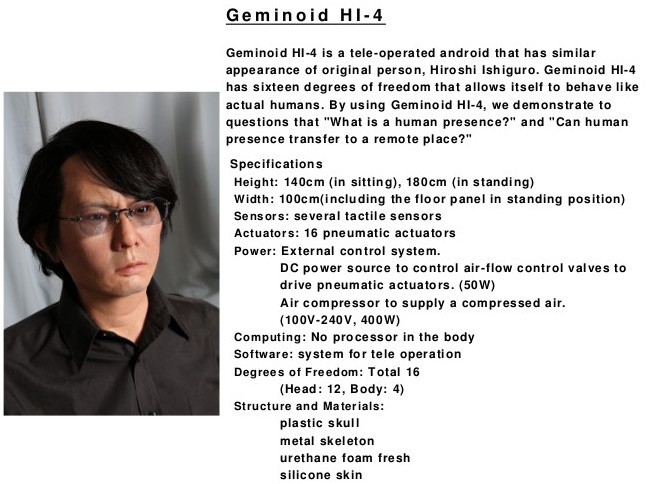
\includegraphics[width=0.95\textwidth]{data/geminoid-HI4}
    \caption{Geminoïde HI-4}
  \end{figure}
  ``Understanding and Transmitting Human Presence''\\
\end{frame}

\begin{frame}{Geminoide HI-2}
  \begin{figure}
    \centering
    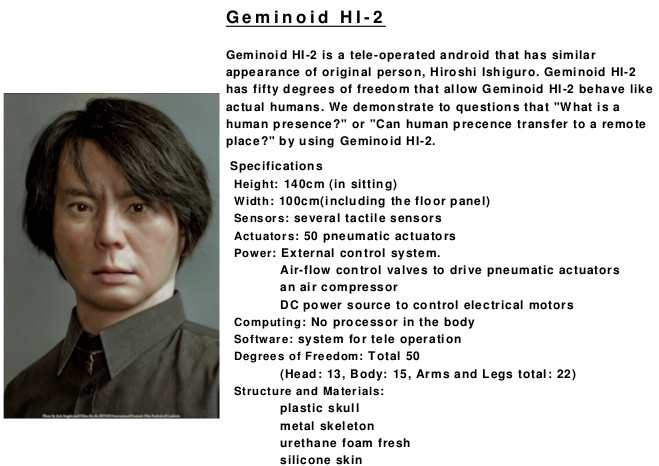
\includegraphics[width=\textwidth]{data/geminoid-HI2}
    \caption{Geminoïde HI-2}
  \end{figure}
\end{frame}

\begin{frame}{Geminoide F}
  \begin{figure}
    \centering
    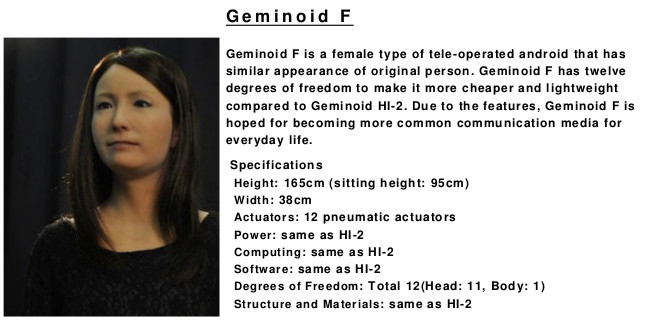
\includegraphics[width=\textwidth]{data/geminoid-F}
    \caption{Geminoïde F}
  \end{figure}
  il y a aussi le DK...\\
  convention social $\rightarrow$ uniquement physique
\end{frame}

\subsection{Conclusion}
\begin{frame}{Un amalgame homme/geminoïde ?}
  \begin{itemize}
  \item l'homme est un moule
  \item 3 videos d'illustrations
  \item les limites de la représentation de l'homme
  \end{itemize}
\end{frame}

\section{L'intéraction}
\begin{frame}{INTERACTIONS}
  \begin{figure}
    \centering
    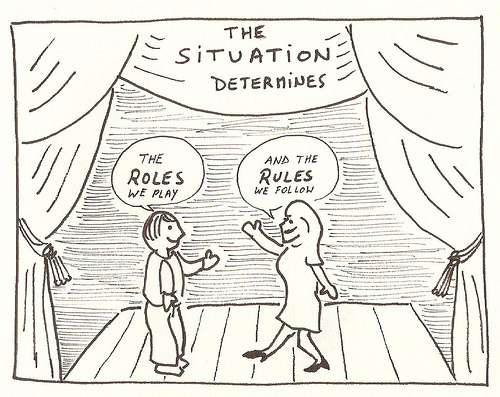
\includegraphics[width=\textwidth]{data/interaction}
    \caption{Le robot Telenoide}
  \end{figure}
\end{frame}

\subsection{Télénoïde}
\begin{frame}{Présentation}
  \begin{figure}
    \centering
    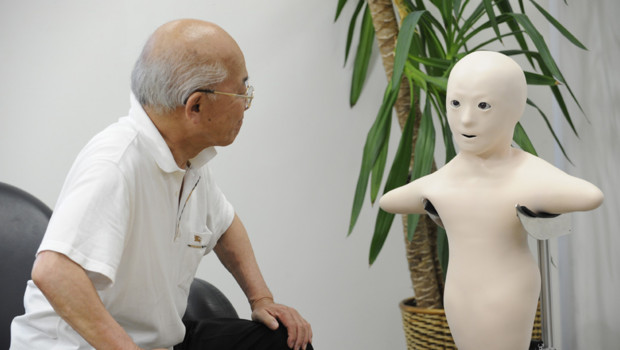
\includegraphics[width=50mm]{data/telenoid}
    \caption{Le robot Telenoide}
  \end{figure}
  Le robot qui transfère votre présence
\end{frame}

\begin{frame}{Caractéristiques}
  \begin{itemize}
  \item 7 versions (depuis aout 2010)
  \item taille : 50cm
  \item poids : 3.5kg
  \item capteurs : 2 microphones
  \item alimentation : batterie
  \item degré de liberté
    \begin{itemize}
    \item 3 sur les yeux
    \item 1 sur la bouche
    \item 3 sur le coup
    \item 2 sur les moignons
    \end{itemize}
  \item peau en PVC
  \item prix 35.000\$ les premiers (environ 8.000\$ desormais)
  \end{itemize}
\end{frame}

\subsection{Utilité}
\begin{frame}
  Design androgyne pour permettre la diversité des utilisateurs.
  \\~\\
  Pas encore assez de capteurs.
  \\~\\
  C'est un téléphone qui a pour but de retransmettre l'idée présence.
  \\
  \begin{itemize}
  \item accueil hotel/aéroport
  \item sex-symbol
  \item ...
  \end{itemize}
\end{frame}

\begin{frame}{Avenir}
  Le robot qui nous permettra l'ubiquité\\
  %\movie[showcontrols]{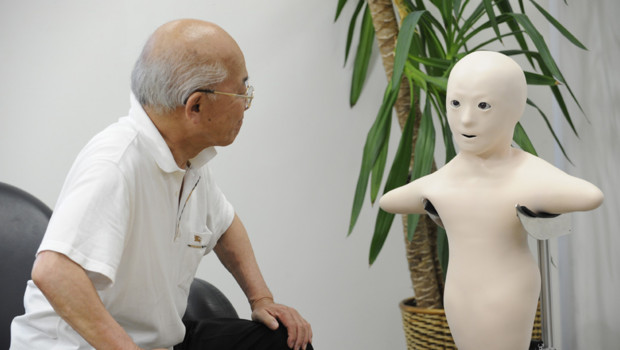
\includegraphics[width=0.8\textwidth]{data/telenoid}}{data/Telenoid_in_action.mp4}
  %\movie[label=cells,width=4cm,height=3cm,poster,showcontrols,duration=5s]{}{data/Telenoid_in_action.mp4}
  %(\href{run:mplayer data/Telenoid_in_action.mp4}{VIDEO})
  \movie[label=cells,width=4cm,height=3cm,externalviewer,showcontrols]{VIDEO}{data/Telenoid_in_action.mp4}
\end{frame}

\subsection{Conclusion}
\begin{frame}{Conclusion}
  \begin{wrapfigure}{l}{50mm}
    \centering
    \vspace*{-3cm}
    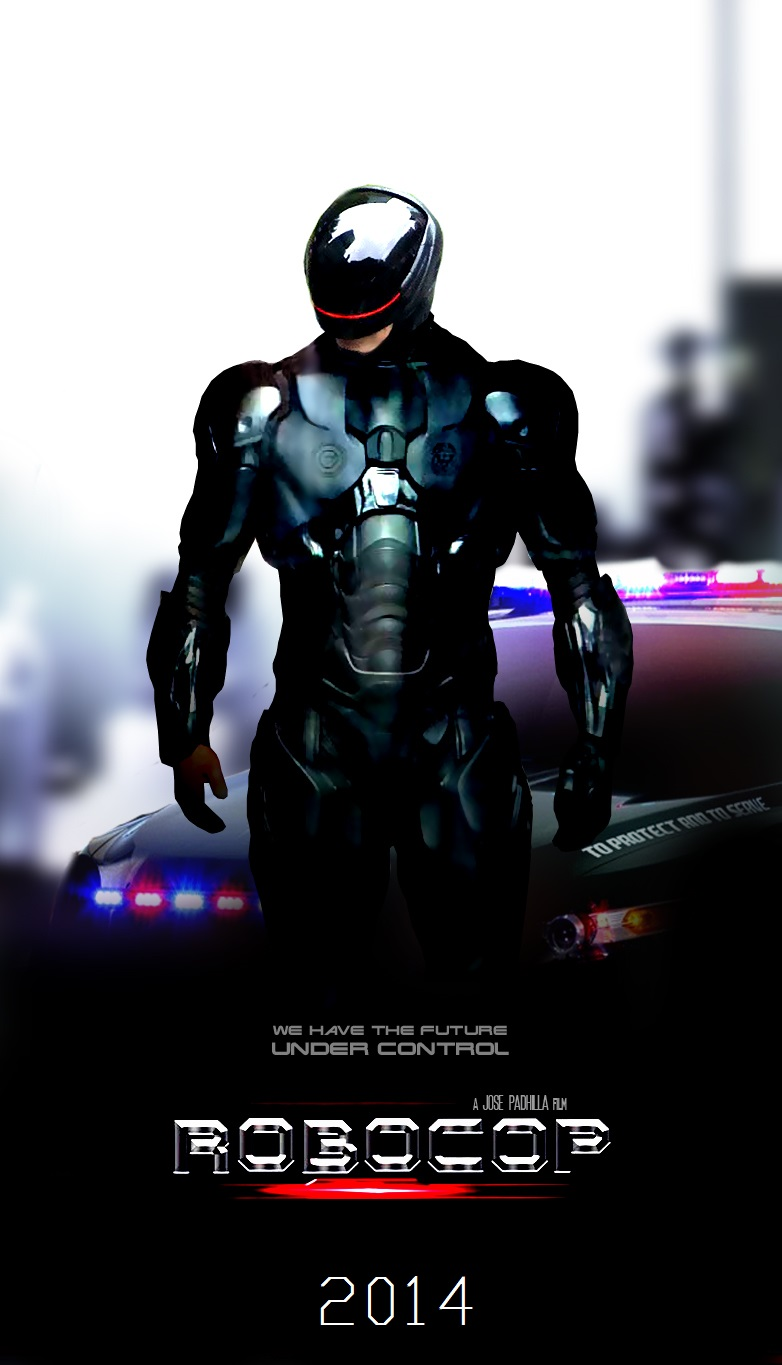
\includegraphics[width=50mm]{data/robocop}
  \end{wrapfigure}
  Réponse floue. Doit connaître les conventions sociales, mais 
  doit-il toutes les appliquées ?
  \begin{itemize}
  \item OUI $\Rightarrow$ complexité, intelligence et peur
  \item NON $\Rightarrow$ pas d'amalgame, efficacité mis en valeur
  \end{itemize}
\end{frame}

\end{document}
